\section{State Space Models are Structured Matrices}
\label{sec:ssm}


This section explores different perspectives of the state space model as a sequence transformation, and outlines properties and algorithms of such maps.
The main results of this section are about the equivalence between state space models and a family of structured matrices called semiseparable matrices,
which imply new efficiency results (\cref{thm:ssm-sss,thm:ssm-efficiency}).

\subsection{The Matrix Transformation Form of State Space Models}

Recall that our definition of an SSM is defined as a parameterized map
defined through \eqref{eq:s6}.
Our theoretical framework starts by simply writing this transformation as a matrix multiplication mapping the vectors $x \in \R^\mathtt{T} \mapsto y \in \R^\mathtt{T}$.

By definition, $h_0 = B_0 x_0$.
By induction,
\begin{align*}
  h_t &= A_t \dots A_1 B_0 x_0 + A_t \dots A_2 B_1 x_1 + \dots + A_t A_{t-1} B_{t-2} x_{t-2} + A_t B_{t-1} x_{t-1} + B_t x_t
    \\&= \sum_{s=0}^t A_{t:s}^\times B_s x_s
    .
\end{align*}

Multiplying by $C_t$ to produce $y_t$ and vectorizing the equation over $t \in [\mathtt{T}]$,
we derive the matrix transformation form of SSMs.
\begin{equation}
  \label{eq:ssm-matrix}
  \begin{aligned}
    y_t &= \sum_{s=0}^t C_t^{\top} A_{t:s}^\times B_s x_s
    \\
    y &= \mathsf{SSM}(A, B, C)(x) = Mx
    \\
    M_{ji} &\coloneqq C_j^{\top} A_{j} \cdots A_{i+1} B_{i}
  \end{aligned}
\end{equation}

\subsection{Semiseparable Matrices}

$M$ in equation \eqref{eq:ssm-matrix} is a particular representation of a class of matrices known as semiseparable matrices.
Semiseparable matrices are a fundamental matrix structure.
We first define these matrices and their properties.

\begin{definition}
  \label{def:semiseparable-rank}
  A (lower triangular) matrix $M$ is $\mathtt{N}$-semiseparable if every submatrix contained in the lower triangular portion (i.e.\ on or below the diagonal) has rank at most $\mathtt{N}$.
  We call $\mathtt{N}$ the \emph{order} or \emph{rank} of the semiseparable matrix.
\end{definition}

\cref{def:semiseparable-rank}, and other forms of related ``separable'' structure (e.g.\ quasiseparable matrices and other definitions of semiseparable matrices) are sometimes called \textbf{structured rank matrices} (or rank-structured matrices) because they are characterized by rank conditions on their submatrices.
Semiseparable matrices have many structured representations including the hierarchical semiseparable (HSS),
sequential semiseparable (SSS), and Bruhat forms~\citep{pernet2018time}.
We will primarily use the SSS form.

\subsubsection{The Sequentially Semiseparable (SSS) Representation}

\begin{definition}
  \label{def:sss}
  A lower triangular matrix $M \in \R^{\mathtt{(T,T)}}$ has a $\mathtt{N}$-\textbf{sequentially semiseparable (SSS)} representation if it can be written in the form
  \begin{equation}%
    \label{eq:sss}
    M_{ji} = C_j^{\top} A_{j} \cdots A_{i+1} B_{i}
  \end{equation}
  for vectors $B_{0}, \dots, B_{\mathtt{T}-1}, C_{0}, \dots, C_{\mathtt{T}-1} \in \R^{\mathtt{N}}$
  and matrices $A_{0}, \dots, A_{\mathtt{T}-1} \in \R^{\mathtt{(N,N)}}$.

  We define the operator $\mathsf{SSS}$ so that $M = \mathsf{SSS}(A_{0:\mathtt{T}}, B_{0:\mathtt{T}}, C_{0:\mathtt{T}})$.
\end{definition}

A fundamental result of semiseparable matrices is that they are exactly equivalent to matrices with SSS representations.
One direction can be deduced with a simple constructive proof.

\begin{lemma}
  \label{lmm:sss-rank-factor}
  An $\mathtt{N}$-SSS matrix $M$ with representation \eqref{eq:sss} is $\mathtt{N}$-semiseparable.
\end{lemma}
\begin{proof}
  Consider any off-diagonal block $M_{j:j', i':i}$ where $j' > j \ge i > i'$.
  This has an explicit rank-$\mathtt{N}$ factorization as
  \begin{equation}
    \label{eq:sss-rank-factor}
    \begin{bmatrix}
      C_j^{\top} A_{j:i'}^\times B_{i'}         & \dots & C_j^{\top} A_{j:i-1}^\times B_{i-1}   \\
      \vdots                                    &       &       \vdots      \\
      C_{j'-1}^{\top} A_{j'-1:i'}^\times B_{i'} & \dots & C_{j'-1}^{\top} A_{j'-1:i-1}^\times B_{i-1} \\
    \end{bmatrix}
    =
    \begin{bmatrix} C_j^{\top} A_{j:j}^\times \\ \vdots \\ C_{j'-1}^{\top} A_{j'-1:j}^\times \end{bmatrix}
    A_{j:i-1}^\times
    \begin{bmatrix} A_{i-1:i'}^\times B_{i'} & \cdots & A_{i-1:i-1}^\times B_{i-1} \end{bmatrix}
    .
  \end{equation}
\end{proof}
Equation \eqref{eq:sss-rank-factor} will be used extensively in deriving our fast algorithms for sequence models.
The other direction is well-established in the literature on semiseparable matrices.

\begin{proposition}
  \label{prop:sss}
  Every $\mathtt{N}$-semiseparable matrix has a $\mathtt{N}$-SSS representation.
\end{proposition}
Furthermore, note that although \cref{def:sss} involves $O(\mathtt{N}^2\mathtt{T})$ parameters for the representation (in particular to store the $A$ matrices),
it can actually be compressed down to $O(\mathtt{NT})$ parameters, which is asymptotically tight~\citep{pernet2023exact}.
Therefore in the rest of this paper we will conflate the structured matrix class (\cref{def:semiseparable-rank}) and a particular representation of it (\cref{def:sss}); we will always use this representation instead of other candidates.
In turn we will use $\mathtt{N}$-SS to refer to an $\mathtt{N}$-semiseparable matrix in SSS form.

Semiseparable matrices are a fundamental matrix structure and have many important properties.
They are deeply related to recurrences at large, and can be defined by multiple characterizations (e.g.\ \cref{def:semiseparable-rank,def:sss}) which reveal different connections and efficient algorithms for them.
We mention some of their other properties in \cref{sec:ssm:properties}.

\begin{remark}
  The notion of semiseparability is very broad and many similar but subtlely different definitions appear in the literature;
  our definitions may differ slightly from other conventions.
  First, because we are primarily concerned with causal or autoregressive settings in this paper,
  we have restricted the definition of semiseparability to the triangular case;
  \cref{def:semiseparable-rank} more formally might be called $(\mathtt{N},0)$-semiseparability by some authors.
  Some authors may also instead refer to it as a form of quasiseparability~\citep{eidelman1999new,pernet2016computing}.
  See \citet{vandebril2005bibliography} for a brief survey.
\end{remark}

\subsubsection{1-Semiseparable Matrices: the Scalar SSM Recurrence}
\label{sec:ssm:1-ss}

We will single out the special case of $1$-SS matrices.
Note that in this case, the $C_j$ and $B_i$ are scalars, and can be factored out of the SSS representation \eqref{eq:sss}
(we also use lower-case to emphasize that the parameters are scalars in this case)
\begin{align*}%
  \mathsf{SSS}(a, b, c) = \mathsf{diag}(c) \cdot M \cdot \mathsf{diag}(b) \qquad \text{where} \qquad M_{ji} = a_{j:i}^\times
  .
\end{align*}

Since diagonal matrices are easy to handle (e.g.\ multiplication by a diagonal matrix is the same as elementwise scalar multiplication),
we can ignore these terms.
Thus our basic representation of a 1-SS matrix is $M_{ji} = a_{j:i}$ or
\begin{equation}%
  \label{eq:1ss}
  M =
  \mathsf{1SS}(a_{0:T}) \coloneqq
  \begin{bmatrix}
    1 & \\
    a_1 & 1 & \\
    a_2a_1 & a_2 & 1 \\
    \vdots & \vdots & \ddots & \ddots \\
    a_{T-1}\dots a_1 & a_{T-1}\dots a_2 & \dots & a_{T-1} & 1 \\
  \end{bmatrix}
  .
\end{equation}

The importance of 1-SS matrices lies in their equivalence to the minimal form of a scalar recurrence -- the case of a degenerate SSM with state dimension $\mathtt{N}=1$ and no $(B, C)$ projections.
Note that multiplication $y = Mx$ can be computed by the recurrence
\begin{equation}
  \label{eq:1ss-recurrence}
  \begin{aligned}
    y_t &= a_{t:0}x_0 + \dots + a_{t:t}x_t \\
        &= a_t \left(a_{t-1:0}x_0 + \dots + a_{t-1:t-1}x_{t-1}\right) + a_{t:t}x_t \\
        &= a_t y_{t-1} + x_t
        .
  \end{aligned}
\end{equation}
We thus also refer to matrix multiplication by $1$-SS matrices as the \textbf{scalar SSM recurrence} or the \texttt{cumprodsum} (cumulative product sum; a generalization of cumulative product and cumulative sum) operator.
As the fundamental form of recurrence, multiplication by 1-SS matrices is important
as a building block for our main algorithms.

We emphasize that one of the central themes of this paper is that \emph{many algorithms on sequence models can be reduced to structured matrix multiplication algorithms}.
1-SS matrices exemplify this connection: there are many fast algorithms for computing the primitive scalar recurrence or \texttt{cumprodsum} operator,
and all of them turn out to be equivalent to different structured factorization of 1-SS matrices.
We dedicate \cref{sec:scan} to these algorithms for 1-SS matrix multiplication.

\subsection{State Space Models are Semiseparable Matrices}
Recall that our definition of an SSM is defined as a parameterized map
defined through \cref{def:sequence-transformation}.
The connection between SSMs and semiseparable matrices follows from simply writing this transformation as a matrix multiplication mapping the vectors $x \mapsto y \in \R^\mathtt{T}$.

Equation \eqref{eq:ssm-matrix} directly establishes the link between state space models and the sequentially semiseparable representation, which in turn are equivalent to semiseparable matrices in general (\cref{lmm:sss-rank-factor,prop:sss}).
\begin{theorem}
  \label{thm:ssm-sss}
  The state space model transformation $y = \mathsf{SSM}(A, B, C)(x)$ with state size $\mathtt{N}$ is identical to matrix multiplication by an $\mathtt{N}$-SS matrix in sequentially semiseparable representation $y = \mathsf{SSS}(A, B, C) \cdot x$.
\end{theorem}

In other words the sequence transformation operator $\mathsf{SSM}$ (\cref{def:ssm}) coincides with the matrix construction operator $\mathsf{SSS}$ (\cref{def:sss}),
and we use them interchangeably (or sometimes $\mathsf{SS}$ as shorthand).
Furthermore---by a twist of fate---structured state space models and sequentially semiseparable matrices have the same acronyms, underscoring their equivalence!
Conveniently we can use any of these acronyms SSM (state space model or semiseparable matrix), SSS (structured state space or sequentially semiseparable), or SS (state space or semiseparable) interchangeably to unambiguously refer to either concept.
However, we will generally use the convention that SSM refers to state space model, SS refers to semiseparable, and SSS refers to sequentially semiseparable.


\cref{fig:ssm-semiseparable} illustrates the sequence transformation perspective of state space models as semiseparable matrices.
\begin{figure}[!t]
  \centering
  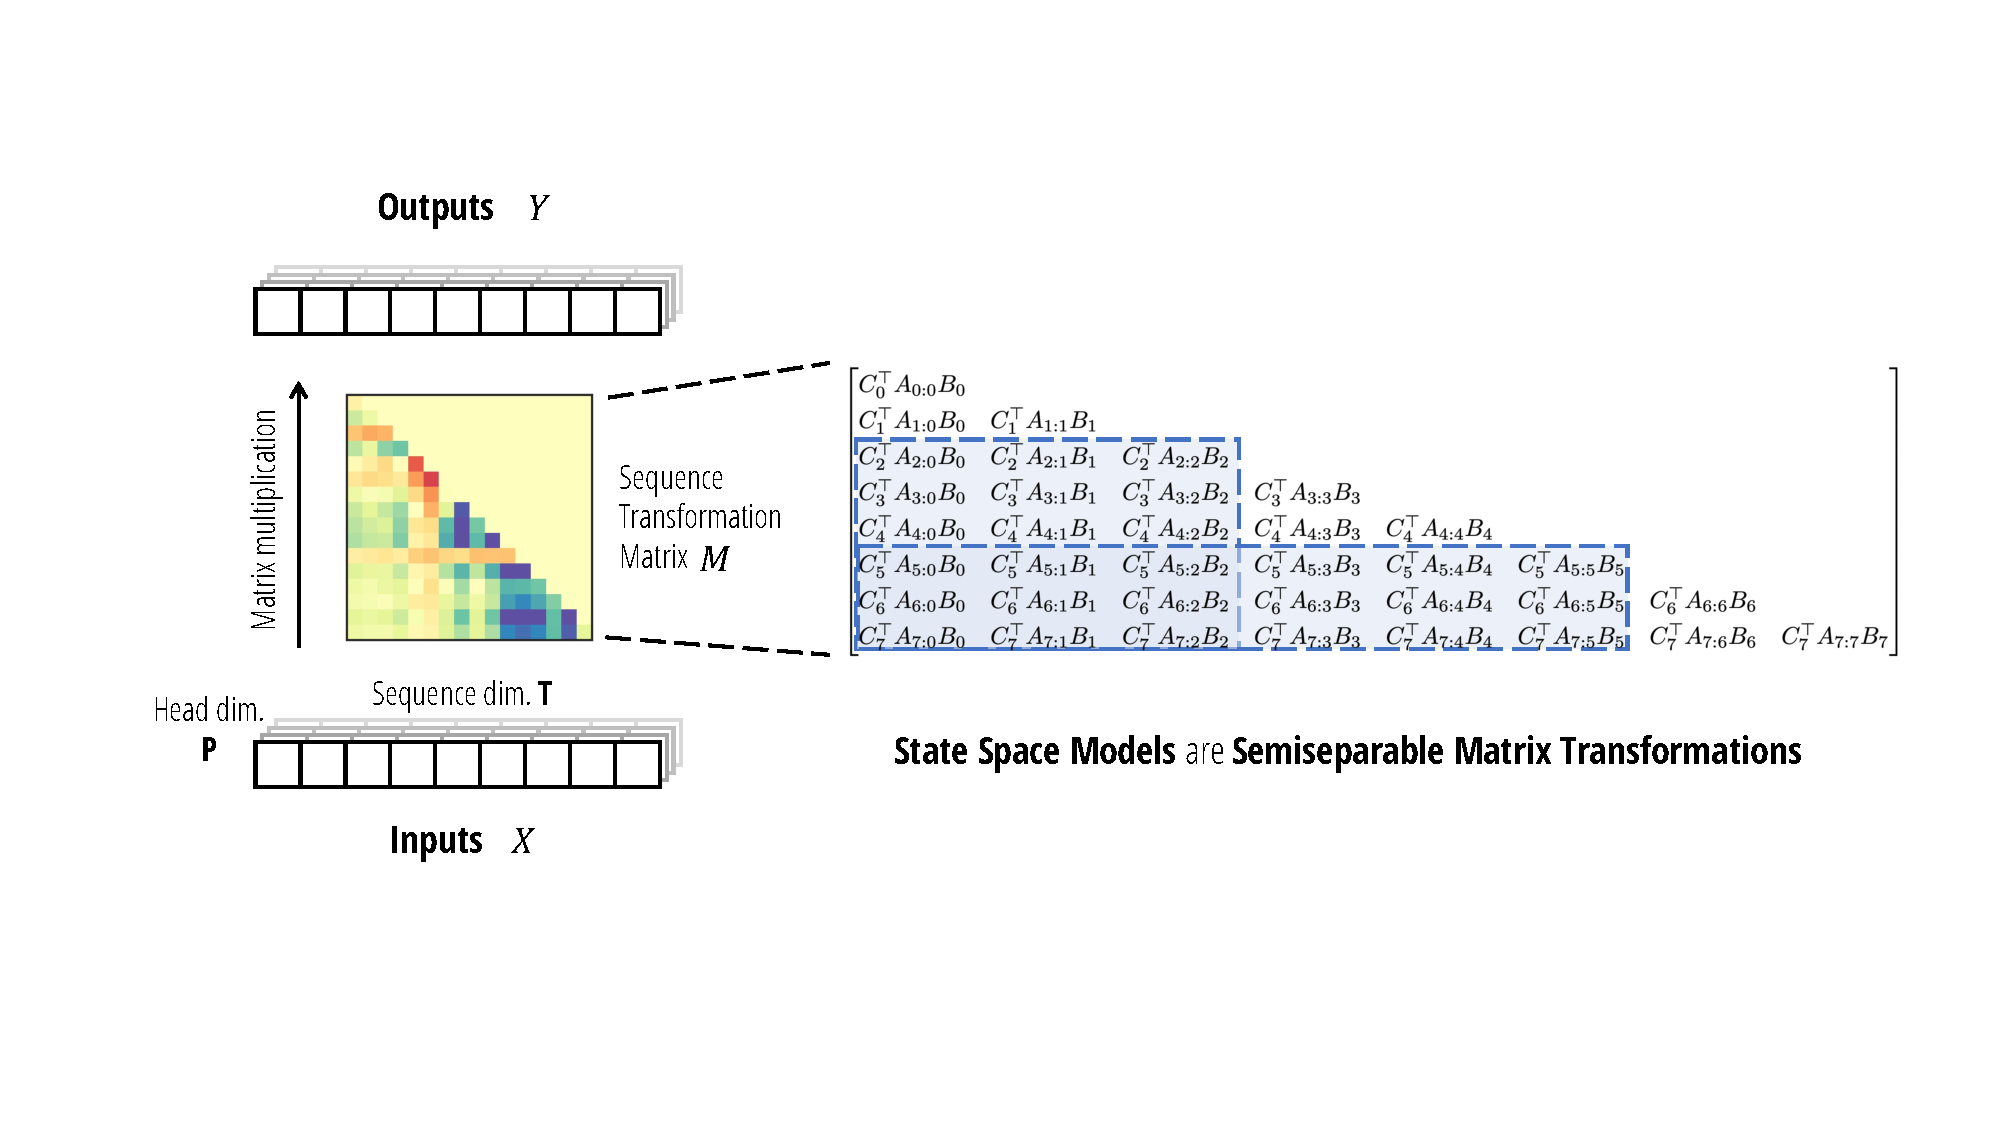
\includegraphics[width=\linewidth]{fig/semiseparable.pdf}
  \caption{
    (\textbf{State Space Models are Semiseparable Matrices}.)
    As sequence transformations, state space models can be represented as a matrix transformation $M \in \mathbb{R}^{\mathtt{(T,T)}}$ acting on the sequence dimension $\mathtt{T}$,
    sharing the same matrix for each channel in a head (\emph{Left}).
    This matrix is a semiseparable matrix (\emph{Right}), which is a rank-structured matrix where every submatrix contained on-and-below the diagonal (\emph{Blue}) has rank at most $\mathtt{N}$,
    equal to the SSM's state dimension.
  }
  \label{fig:ssm-semiseparable}
\end{figure}


\subsection{Computing State Space Models through Structured Matrix Algorithms}
\label{sec:ssm:algorithms}

The reason \cref{thm:ssm-sss} is important is that it will allow us to \emph{reduce the problem of efficient computation of SSMs (and other sequence models) into efficient algorithms for structured matrix multiplication}.
We briefly provide an overview and defer our main new algorithm to \cref{sec:efficient}, after showing the equivalence of SSMs to other sequence models in
\cref{sec:attention,sec:ssd}.

As previously defined, semiseparable matrices (i.e.\ rank-structured matrices) are a classical type of structured matrix:
\begin{enumerate}[label=(\roman*)]
  \item They have compressed representations such as the SSS form which has only $O(\mathtt{T})$ instead of $O(\mathtt{T}^2)$ parameters.
  \item They have fast algorithms operating directly on the compressed representation.
\end{enumerate}
Furthermore, the parameterization and matrix multiplication cost can be tight in the semiseparable order.
\begin{proposition}[\citet{pernet2023exact}]
  \label{prop:ss-mvm}
  An $\mathtt{N}$-SS matrix of size $\mathtt{T}$ can be represented in $O(\mathtt{NT})$ parameters and has matrix-vector multiplication in time and space $O(\mathtt{NT})$.
\end{proposition}

For example, 1-SS matrices illustrate the essence of this connection.
The matrix $M = \mathsf{1SS}(a)$ is defined by exactly $\mathtt{T}-1$ parameters $a_{0:\mathtt{T}-1} = a_1, \dots, a_{\mathtt{T}-1}$,
and can be computed in $O(\mathtt{T})$ time by following the scalar recurrence \eqref{eq:1ss-recurrence}.




\subsubsection{The Linear (Recurrent) Mode}
\label{sec:ssm:algorithms:linear}

\cref{prop:ss-mvm} can be easily seen in the case of diagonal structured SSMs (S4D~\citep{gu2022parameterization}),
simply by leveraging the state space model formulation \eqref{eq:s6} and unrolling the recurrence.
We provide the formal tensor-contraction algorithm in \eqref{eq:ssm-diagonal}, where the dimension $\mathtt{S}$ is equal to $\mathtt{T}$%
\footnote{A different symbol is required for the contraction notation.}.
\begin{subequations}
  \label{eq:ssm-diagonal}
  \begin{align}
    \label{eq:ssm-diagonal:1}
    Z &= \mathsf{contract}(\mathtt{SP},\mathtt{SN} \to \mathtt{SPN})(X, B) & \mathtt{(S,P,N)} \\
    \label{eq:ssm-diagonal:2}
    H &= \mathsf{contract}(\mathtt{TSN},\mathtt{SPN} \to \mathtt{TPN})(L, Z) & \mathtt{(T,P,N)} \\
    \label{eq:ssm-diagonal:3}
    Y &= \mathsf{contract}(\mathtt{TN},\mathtt{TPN} \to \mathtt{TP})(C, H) & \mathtt{(T,P)}
  \end{align}
\end{subequations}
Here, $L \in \R^{(\mathtt{T},\mathtt{T})}$ is defined as $\mathsf{1SS}(A)$, or in other words $L_{0:\mathtt{T},0:\mathtt{T}} = \mathsf{1SS}(A_{0:\mathtt{T}})$ for $i \in [\mathtt{N}]$.
This algorithm involves three steps corresponding to \eqref{eq:s6}:
\begin{enumerate}[label=(\roman*)]
  \item \emph{expanding} the input $X$ by the input matrix $B$ \eqref{eq:ssm-diagonal:1},
  \item unrolling independent scalar SSM recurrences \eqref{eq:ssm-diagonal:2}, and
  \item \emph{contracting} the hidden state $H$ by the output matrix $C$ \eqref{eq:ssm-diagonal:3}.
\end{enumerate}
Note that we have used the equivalence between scalar SSMs and 1-SS matrices in step \eqref{eq:ssm-diagonal:2}.

\begin{remark}
  We note that \eqref{eq:ssm-diagonal} is a special case of the Mamba (S6) model.
  however, a naive implementation is slow because of the expanded tensors $Z$ and $H$ of size $\mathtt{(T,P,N)}$;
  \citet{gu2023mamba} introduced a hardware-aware implementation to avoid materializing these tensors.
\end{remark}



Surprisingly, \cref{thm:ssm-sss} and \cref{prop:ss-mvm} immediately imply that all SSMs have the same asymptotic efficiency as algorithm \eqref{eq:ssm-diagonal}.
\begin{theorem}
  \label{thm:ssm-efficiency}
  Any state space model (\cref{def:ssm}) of state size $\mathtt{N}$ on sequence length $\mathtt{T}$ can be computed in time $O(\mathtt{TN})$ (not accounting for potential preprocessing).
\end{theorem}
We note that this result is new to the structured SSM literature.
In particular, given dense unstructured $A_t$ matrices, the total representation alone seems to be of size $O(\mathtt{TN}^2)$.
Thus \cref{thm:ssm-efficiency} states the non-trivial result that with a pre-processing step, even an unstructured SSM can be computed optimally efficiently,
with upper bound matching the lower bound $O(\mathtt{TN})$ given by the size of $B$ and $C$.

\begin{remark}
  \cref{thm:ssm-efficiency} is perhaps not too surprising in light of the fact that almost all dense matrices over $\R^{\mathtt{(N,N)}}$ are diagonalizable over $\mathbb{C}$,
  leading to the result that \emph{almost all} dense real SSMs are equivalent to a diagonal complex SSM.
  This fact underlies the reason why diagonal SSMs are the most popular form of structured SSM~\citep{gupta2022diagonal,gu2022parameterization,smith2023s5}.
  However, \cref{thm:ssm-efficiency} implies the much stronger result for \emph{all} real SSMs (not just the diagonalizable ones), as well as dense SSMs over other fields (including $\mathbb{C}$ itself).
\end{remark}

In practice, efficiently computable SSMs still require additional structure on $A$,
particularly to avoid the expensive preprocessing step (which both has order $\mathtt{N}$ extra FLOPs and involves hardware-inefficient operations such as singular value decompositions).
These structures are the focus of past work on structured SSMs (e.g.\ S4(D) and Mamba) as well as our new algorithms.
In particular, when slightly stronger structure is imposed on $A$, we will design very hardware-efficient algorithms through block decompositions of the SSM matrix $M = \mathsf{SSS}(A, B, C)$ in \cref{sec:efficient}.

\subsubsection{The Quadratic (Naive) Mode}

We note that there is another way to compute an SSM exposed by our new matrix point of view.
A naive computation of the matrix SSM representation \eqref{eq:ssm-matrix} involves simply materializing the sequence transformation matrix $M=\mathsf{SSS}(A, B, C)$.
This is a $\mathtt{(T,T)}$ matrix, and therefore this naive algorithm will scale quadratically in sequence length.
However, when the sequence length $\mathtt{T}$ is short, this can actually be more efficient than the linear algorithm due to constant factors and the hardware-friendliness of the computation pattern (e.g. leveraging matrix-matrix multiplications).
In fact, for a particular case of structured SSMs, this looks very similar to a quadratic attention computation (\cref{sec:ssd}).




\subsubsection{Summary}

Many sequence models are explicitly motivated or defined as matrix sequence transformations --
most notably Transformers, where the matrix mixer is the attention matrix.
On the other hand, RNNs and SSMs have not previously been described in this way.
By providing an explicit \emph{matrix transformation} form of state space models,
we reveal new ways of understanding and using them.
From a computational perspective, any method of computing the forward pass of a state space model can be
viewed as a matrix multiplication algorithm on semiseparable matrices.
The semiseparable matrix perspective provides one lens into state space duality (SSD),
where the dual modes respectively refer to a linear-time semiseparable matrix multiplication algorithm and quadratic-time naive matrix multiplication.

Moreover, leveraging the rich structure of semiseparable matrices can lead to even better algorithms and more insights (e.g. \cref{sec:efficient,sec:scan}).
In \cref{sec:ssm:properties}, we describe some additional properties of semiseparable matrices.


